\documentclass[10pt]{article}
\usepackage[margin=.7in]{geometry}
\usepackage{amsthm}
\usepackage{hyperref}
\usepackage{graphicx}
\usepackage{booktabs}
\listfiles

\begin{document}
 
\begin{center}
\large
\hfill Okeefe Niemann\\
\hfill 5/31/2014\\
\hfill 1281465\\
\hfill PHYS 115 \\
\LARGE \textbf{Ising Model by Monte Carlo Method}\\
\end{center}
\normalsize
\section{Introduction}
When a molecular system is connected to a heat reservoir, the state of the system can be statistically represented by:

\begin{equation}
P(n) = \frac{1}{Z} e^{-\frac{E_n}{k_B T}}
\end{equation}
where the normalizing factor $Z$ corresponds to the partition function of the system.

$$Z = \sum\limits_{l} e^{-\frac{E_l}{k_B T}}$$
This factor connects the macroscopic qualities (thermodynamics) to the microscopic qualities involving the states and their corresponding energy levels. From this, it's possible to calculate observable variables as averages over states with a Boltzmann weight. Compiling this all together, it is then simple to calculate the average value of a quantity over all states.

\begin{equation}
<A>  =  \sum\limits_{n} P(n)A_n  =  \frac{\sum\limits_{n} A_n e^{-\frac{E_l}{k_B T}}}{\sum\limits_{l} e^{-\frac{E_l}{k_B T}}}
\end{equation}

In the ising model for magnetism, the magnetic moment of an atom can be represented by ``up'' (+1) and ``down'' (-1). If there are N spins in the lattice, there are $2^N$ states in which the system can exist, and the distribution of possible states can be represented as a binomial distribution if comparing it to the spin imbalance factor k. Furthermore, if the number of states goes to an arbitrarily large number, these range of states begin to represent a gaussian distribution. If one continues to statistically analyze the properties of magnetization per spin of a lattice, the individual will find that the probability that a system which is not self-interacting (ie where the spins are independent of each other) has a particular value of magnetization per spin which is dependent on the total Boltzmann weight of all states with that value of m.

\begin{equation}
P(m)\hspace{1mm}\alpha\hspace{1mm}exp[-N(\frac{m^2}{2} - \beta hm)]
\end{equation}
Here, h corresponds to the magnetic field applied to the lattice and $\beta = k_B T$. From this value of P(m), we see that as $T \to \infty$, which corresponds to an equal weighting in all states, a system tends to magnetization per spin of 0. On the other hand, at finite T, a large system tends to states which have m close to a particular value $m* = \beta h$. Extrapolating this idea to a self-interacting system, we find that the general idea holds true. At infinite temperature, the states available to the system will have energy close to a certain value, while at a finite temperature, the system will tend to states with energy in the vicinity of a different value of m.

For this project, the Ising model of magnetism will be used to show this statistical interpretation of a system connected to a reservoir. Each of the spins will be interacting with each other, so it becomes energy dependent on the orientation of them within the lattice. 

\begin{equation}
\mathcal{H} = - J \sum\limits_{<i,j>} S_i S_j - \sum\limits_{i} S_i
\end{equation}
For the purposes of the project, $J > 0$ will be considered (specifically $J=1$), where the system is ferromagnetic due to the tendency of the spins to align parallel with each other at low temperatures. For a theoretical infinite lattice, the average magnetization per spin of the system will be zero above a critical temperature $T_C$. Below this temperature, $<m^2>$ will begin to rise as the particles align themselves until this value achieves unity. This transition is what I will be modeling with sample sizes of an infinite lattice. 

Using the Monte Carlo technique, states which satisfy the Boltzmann distribution will be randomly generated by virtue of the ``detailed balance condition'', which states that the ratio of the system being in two different states at time t.


$$\frac{P^{eq}_m}{P^{eq}_l} = exp\left(\beta{E_m-E_l)\right)$$
With the above, we can determine the probability of transition from the spin up state to the spin down state by the Metropolis updating probability.

\begin{displaymath}
  w_{l \to m} = \left\{
    \begin{array}{lr}
     exp\left(\beta(E_m-E_l)\right), \hspace{2mm} E_m - E_l > 0\\
     1, \hspace{27mm} otherwise
    \end{array}
  \right.
\end{displaymath}

\section{Program}
In the following simulations, $J = k_B = 1$ and the energy will be given by the first term in equation (4), where the sum is over all nearest neighbor pairs on the lattice. The phase transition temperature will be $T_C = 2.269$. 

\begin{verbatim}
#include <stdio.h>
#include <math.h>
#include <time.h>
#include <stdlib.h>
#include "MonteCarlo.h"


int main()
{
        int L, T_RUNS;
        
        printf("How many spins in the lattice? ");
        scanf("%d", &L);
        printf("How many times should we run the Ising model? ");
        scanf("%d", &T_RUNS);
        
        int k, t, i, j, z, val;
        int N = L * L;			 //total number of spins in L x L lattice
        int t_eq = 4 * L * L;		 //number of sweeps for equilibriation period
        int N_UP = 4 * 4 * L * L;	 //number of sweeps for measuring period
        double TMAX = 4; 	         //maximum temperature to be measured
        double T_Crit = 2.269;		 //given critical temperature
        double M_MEAS = N_UP * T_RUNS;   //total times <m^2> is measured for each temperature
        
        double m_sq, m_squ, S[L][L], m_sqavg, m_frth, m_frthavg, E, currentT, r, prob[17];;
        
        srand(time(NULL));	         //initializes random number generator
        
        FILE* fout;
        fout = fopen("isingmodel8.txt", "w");
        
        fprintf(fout, "Temperature   <m^2>     errorbar  errorbarx5  xaxis    yaxis\n");

clock_t start = clock();

for(currentT = 0.01; currentT <= TMAX; currentT += 0.01)
{
        //creates 9 possible values of energy each spin within lattice
        //placed in this location to reduce computation time
        for(val = -8; val <= 8; val+=2)
        {
                prob[val + 8] = exp(-val / currentT);    
        }                                             
        
        initialize(currentT, L, S);                         //initializes lattice
        m_sqavg = 0;
        m_fthavg = 0;

        for(k = 0; k < T_RUNS; k++)                        //loops ising model simulation T_RUNS times
        {
                m_sq = 0;
                
                for(z = 0; z < t_eq; z++)
                        update(L, S, currentT, prob);      //equilibriation period

                for(t = 0; t < N_UP; t++)
                {
                        update(L, S, currentT, prob);       //updates lattice using Monte Carlo technique
                        m_sq = avgmagnetization(N, L, S);   //calculates average magnetization per spin

                        m_squ += m_sq;     	          //calculates m^2 of all updates
                        m_frth += m_sq * m_sq;           //calculates m^4 of all updates
                }
                
                m_sqavg += m_squ / M_MEAS;                   //calculates <m^2> for each temperature
                m_frthavg += m_frth/ M_MEAS;               //calculates <m^4> for each temperature
                }
                
        //prints T, <m^2>, and each error bar 
        fprintf(fout, "%f    %f   %f\n", currentT, m_sqavg / (N*N),
                            sqrt((m_frthavg - m_sqavg * m_sqavg)/(N*N*N*N)) / sqrt(M_MEAS - 1));
        double percentage = currentT / TMAX * 100;
        printf("%.1f%%\n", percentage);
}

clock_t end = clock();
double elapsed_time = (end-start)/(double)CLOCKS_PER_SEC;
printf("Computation Time: %f.3\n", elapsed_time);           //computes time taken to run code

return 0;
}
\end{verbatim}

The first loop is designed to run from $T=0$ to $T=4$ in increments of $0.01$. Then, in order to initialize the lattice of size $N = L\times L$ for the region $T>T_C$, I utilized a random number generator which decided the direction of each spin based on the corresponding random number's deviation from $0.5$. In order to reduce computation time, I predetermined the orientation of the group of parallel spins for $T<T_C$.

\begin{verbatim}
//initializes spin lattice
double initialize(double currentT, int L, double S[L][L])
{
        double T_Crit =2.269;
        int i, j;
        
        if(currentT < T_Crit)               //if T < critical temperature, all spins are parallel
        {
                for(i = 0; i < L; i++)
                {
                        for(j = 0; j < L; j++)
                                S[i][j] = 1.;
                }
        }
        
        else                          //if T > crit temp, randomizes all spins
        {
                for(i = 0; i < L; i++)
                {
                        for(j = 0; j < L; j++)
                        {
                                if(rand() / RAND_MAX < 0.5)
                                        S[i][j] = 1.;
                                else
                                        S[i][j] = -1.;
                        }
                }
        }
}
\end{verbatim}

The lattice will then be in an initial state in which it will be elligible for manipulation via the monte carlo technique. In both the equilibriation period and the measurement period, the energy of the individual spins are given by

$$\Delta E = 2JS_i \sum\limit_{j neighbor of i} S_j$$,
where the sum is over the neighbors of $S_i$. I then generated a number with a uniform distribution between 0 and 1, flipping $S_i$ if

$$r < exp(-\beta \Delta E)$$
In order to increase the efficiency of the program, I predetermined the 9 values of the energy (due to the combinations of possible values of $\Delta E$), stored the values in an array, and called the array when comparing the randomly generated number. Because $S_i$ will always flip if $\Delta E$ is less than zero, the Metropolis probability being used for this model is always satisfied. The ends of the square lattice were taken into account in this updating method, utilizing periodic boundary conditions.

\begin{verbatim}
//updates the lattice, which has periodic boundary conditions for both i and j axes
double update(int L, double S[L][L], double currentT, double prob[17])
{
        int ir, i, il, ju, j, jd, val, E;
        double r;
        
        il = L - 2;
        i = L - 1;
        ju = L - 2;
        j = L - 1;
        
        for(ir = 0; ir < L; ir++)      //loops through, updating each spin state in the lattice
        {
                for(jd = 0; jd < L; jd++)
                {
                        r = rand() / (RAND_MAX + 1.);
                        E = 2 * S[i][j] * (S[ir][j] + S[il][j] + S[i][jd] + S[i][ju]);
                        
                        //compares generated random number to the implemented detailed balance condition
                        if(r < prob[E + 8])
                        {
                                S[i][j] = -S[i][j];
                        }
                        
                        ju = j;
                        j = jd;
                }
                il = i;
                i = ir:
        }
}
\end{verbatim}

The lattice is then updated multiple times during the ''$M_{drop}$`` period, and is then further updated for measurements. All of the direct measurements use the below function, which calculates the average magnetization per spin of the lattice and subsequently the average magnetization squared.

\begin{verbatim}
//calculates the average magnetization of the lattice at any given timestep
double avgmagnetization(int N, int L, double S[L][L]) 
{
        int i, j;
        double m_avg = 0;
        
        for(i = 0; i < L; i++)
                for(j = 0; j < L; j++)
                        m_avg += 1. * S[i][j];
                        
        double m_sq = m_avg * m_avg
       
        return m_sq; 
}
\end{verbatim}
At the end of each measurement period, $<m^2>$ was measured, and subsequently after each repeat of this equilibriation-measurement cycle the array of this value was averaged. Finally, found within the print statement is the standard deviation of $<m^2>$ for each temperature value. Because I only collected sample points, this value is calculated by: 

$$\sigma_\mu = \frac{s}{(M_{meas}-1)^\frac{1}{2}}$$,

where

$$s^2 = \frac{1}{M_{meas}} \sum\limits_{\alpha = 1}^{M_{meas}} \left(X_\alpha - \overline{X}\right)^2 = <X^2> - <X>^2$$

and $M_{meas} = T_{runs} \times N_{up}$. The method for solving the error bars in this program rely on the rightmost equality in the above formula. 

\section{Results}
\subsection*{Question 1}
In running the ising model program shown above, the following results were obtained.

\begin{center}
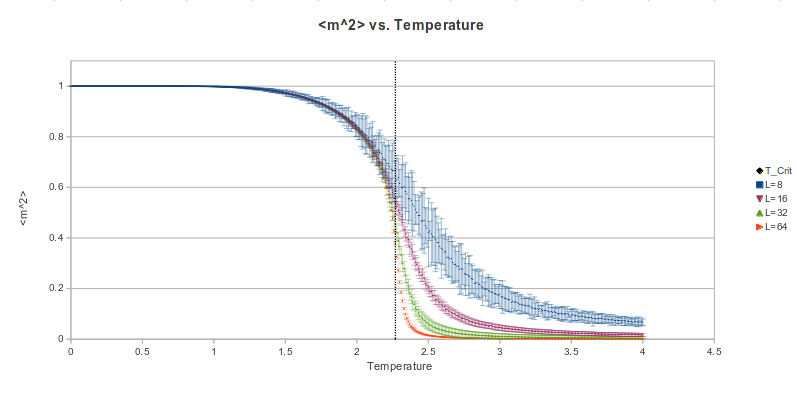
\includegraphics[scale=0.6]{msqvstemp}

\footnotesize $T_{run} = 10$; $t_{eq} = 4L$; $N_{up} = 16L^2$
\end{center}
Above, the dotted black line corresponds to the value of $T_C$, while the error bars correspond to 10$\sigma$ to show the errors more clearly. As expected, increasing the size of the lattice results in a sharper decrease of $<m^2>$ as the system nears $T_C$. This shows that if $N \to \infty$, the average magnetization squared will trunkate at exactly $T_C$. The decrease in the value of the error bars with increasing lattice size is also worth mentioning, showing that a sample size as small as 64 can produce a decently statistical array of data. 

\subsection*{Question2}
The reason $<m>$ was never asked to be calculated was because it trivially evaluates to zero when the ising model is run a large amount of times. This is because the magnetization per spin only has three values: -1, 0, and +1. Averaging these together yields a value of zero.

\subsection*{Question 3}
\begin{center}
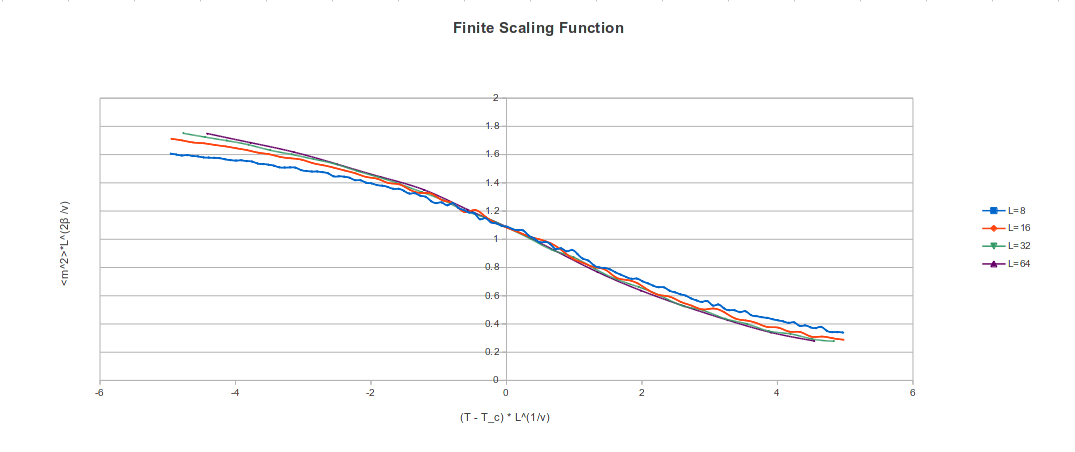
\includegraphics[scale=0.5]{finitescalingfunction}

\footnotesize $\beta = \frac{1}{8}$; $\nu = 1$; $T_C = 2.269$
\end{center}

As seen in the above graph, the data for all the different sized lattices ''collapses`` onto a common curve right at $T=T_C$. This shows that it is actually the correct value, and how we can use multiple sample sizes in order to find this critical temperature to relatively high accuracy.  

\end{document}
